\documentclass{article}

\usepackage{graphicx}
\usepackage{tikz}
\usepackage{tikzsymbols}
\usetikzlibrary{calc,patterns,shapes.geometric}
\pagestyle{empty}
\usepackage[margin=0pt]{geometry}
\geometry{papersize={14in,12in}}

\def\centerarc[#1](#2)(#3:#4:#5){\draw[#1] ($(#2)+({#5*cos(#3)},{#5*sin(#3)})$) arc (#3:#4:#5);}

\begin{document}
	\begin{figure}
		\centering
		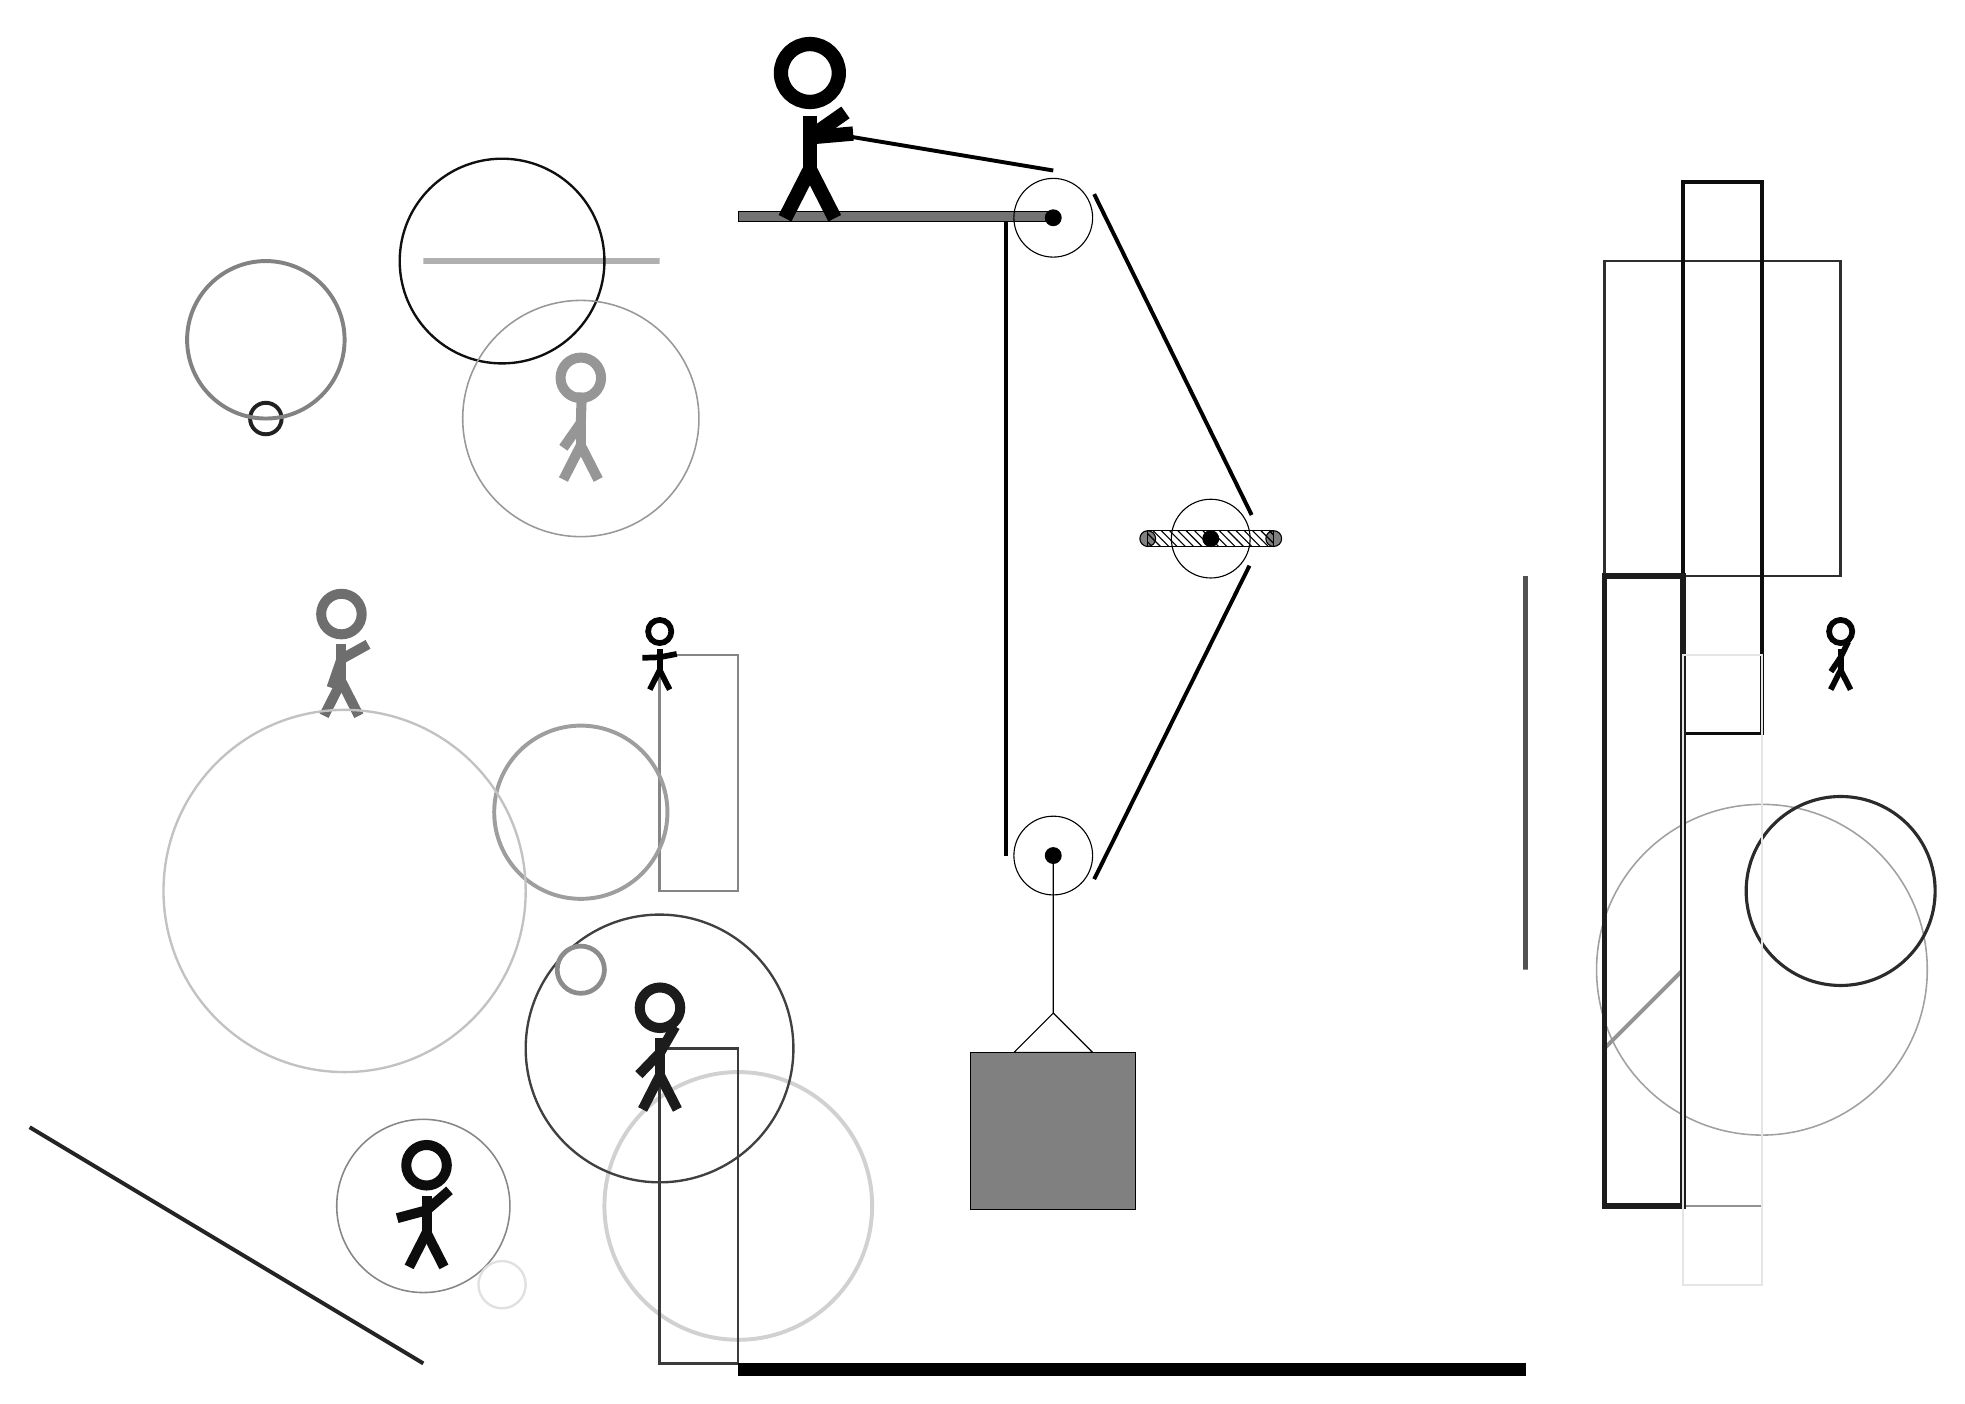
\begin{tikzpicture}
			%%%%% START %%%%%
			
			\draw[fill=black!55] (-2, 11.5) rectangle (2, 11.625);
			
			\draw (2, 3.45) circle (0.5);
			\draw[fill=black] (2, 3.45) circle (0.1);
			
			\draw (2, 11.55) circle (0.5);
			\draw[fill=black] (2, 11.55) circle (0.1);
			
			\draw[fill=white](4, 7.475) circle (0.5);
			\draw[fill=black] (4, 7.475) circle (0.1);
			\draw[fill=black!50] (3.2, 7.475) circle (0.1);
			\draw[fill=black!50] (4.8, 7.475) circle (0.1);
			\draw[pattern=north west lines, pattern color=black] (3.2, 7.575) rectangle (4.8, 7.375);
			
			\draw (2, 3.45) -- (2, 1.45) -- (1.5, 0.95) -- (2.5, 0.95) -- (2, 1.45);
			\draw[fill=black!50] (0.95, 0.95) rectangle (3.05, -1.05);
			
			\draw[line width=0.5mm] (1.4, 11.5) -- (1.4, 3.45);
			\centerarc[line width=0.5mm](2, 3.45)(180:330:0.6);
			\draw[line width=0.5mm](2.5196, 3.15) -- (4.4915, 7.1308);
			\centerarc[line width=0.5mm](4, 7.475)(390:325:0.6);
			\draw[line width=0.5mm](4.5196, 7.775) -- (2.5196, 11.85);
			\centerarc[line width=0.5mm](2, 11.55)(30:90:0.6);
			\draw[line width=0.5mm](2, 12.15) -- (-1, 12.65);
			
			\node at (-1, 12.65) {\Strichmaxerl[10][-175][35]};
			
			\draw[line width=0.3mm, color=black!82] (9, 7) rectangle (12, 11);
			
			\draw[line width=0.6mm, color=black!68] (8, 2) rectangle (8, 7);
			\draw[line width=0.5mm, color=black!95] (10, 5) rectangle (11, 12);
			\draw[line width=0.3mm, color=black!48] (-2, 6) rectangle (-3, 3);
			
			\draw [line width=0.2mm, color=black!47](-6, -1) circle (1.1);
			\node[line width=0.7mm, color=black!41] at (-4, 9) {\Strichmaxerl[7][55][88]};
			\node[line width=0.5mm, color=black!98] at (12, 6) {\Strichmaxerl[4][56][64]};
			\draw[line width=0.7mm, color=black!31] (-3, 11) rectangle (-6, 11);
			\node[line width=0.6mm, color=black!99] at (-3, 6) {\Strichmaxerl[4][2][11]};
			
			\draw [line width=0.5mm, color=black!18](-2, -1) circle (1.7);
			\draw[line width=0.2mm, color=black!43] (10, -2) rectangle (11, -1);
			\draw [line width=0.2mm, color=black!37](11, 2) circle (2.1);
			\draw [line width=0.5mm, color=black!87](-8, 9) circle (0.2);
			\draw [line width=0.3mm, color=black!12](-5, -2) circle (0.3);
			\draw[line width=0.5mm, color=black!86](-6, -3) -- (-11, 0);
			\draw[line width=0.3mm, color=black!77] (-3, 1) rectangle (-2, -3);
			
			\draw[line width=0.5mm, color=black!42](10, 2) -- (9, 1);
			
			\draw [line width=0.3mm, color=black!94](-5, 11) circle (1.3);
			\draw [line width=0.4mm, color=black!83](12, 3) circle (1.2);
			\draw [line width=0.3mm, color=black!75](-3, 1) circle (1.7);
			\draw [line width=0.5mm, color=black!38](-4, 4) circle (1.1);
			\draw[line width=0.7mm, color=black!89] (9, 7) rectangle (10, -1);
			\draw[line width=0.3mm, color=black!10] (10, 6) rectangle (11, -2);
			\node[line width=0.5mm, color=black!89] at (-3, 1) {\Strichmaxerl[7][46][60]};
			\draw [line width=0.5mm, color=black!49](-8, 10) circle (1.0);
			
			\draw [line width=0.2mm, color=black!40](-4, 9) circle (1.5);
			
			\node[line width=0.6mm, color=black!95] at (-6, -1) {\Strichmaxerl[7][15][41]};
			\node[line width=0.4mm, color=black!57] at (-7, 6) {\Strichmaxerl[7][71][29]};
			
			\draw [line width=0.3mm, color=black!24](-7, 3) circle (2.3);
			
			\draw [line width=0.6mm, color=black!45](-4, 2) circle (0.3);
			
			\draw[fill=black] (-2, -3) rectangle (8, -3.15);
			
			%%%%% END %%%%%
		\end{tikzpicture}
	\end{figure}	
\end{document}